%!TEX root = Thesis.tex
\chapter{Implementation and Evaluation}
	The chapter contains practical part of the work, describing implementation of suggested prototype in the section
	2.3. The prototype implements the major aspects proposed in the concept (chapter 4).
	The implementation consists the major aspects proposed in the concept, according to 3-tier architecture. Namely next components:
	 \begin{itemize}
		\item \textbf{Client Tier} presents adaptive to different screens GUI, dynamically changed content and cookies for authorization
		\item \textbf{Application Tier} consists Apache Web-server, XMPP server and guarantee appropriate interface of collaboration between tiers via JSON format and defined structure
		\item \textbf{Data Tier} consists data streaming of map of values, images and text
	\end{itemize}
	To make evaluations real, system will use data from the VICCI(Visual and Interactive Cyber-physical Systems Control and Integration) project at the Faculty of Computer Science of the Dresden University of Technology. The scope includes smart home environments and supporting people in the ambient assisted living. Also it was connected by using Data Hub as a Proxy, that is the part of Master Thesis of Luiz Alberto Borges, "Data Hub for Adaptive Data Services".

\section{Development Environment}
	As a programming languages for implementation of this work jQuery\footnote{jQuery programming language, \url{http://jquery.com/}} and HTML5\footnote{HTML specification, \url{http://www.w3.org/wiki/HTML/Specifications}} together with CSS\footnote{CSS specification, \url{http://www.w3.org/Style/CSS/specs.en.html}} are chosen. jQuery is a fast, small, well documented, easy and widely used and feature-rich JavaScript library. In addition it has such an important properties as: chaining, easy-to-use AJAX, event handlers, CSS selectors, pluins. It makes things like HTML document traversal and manipulation, event handling, animation, and Ajax much simpler with an easy-to-use API that works across a multitude of browsers. It enables the project code to be portable over different platforms and provides opportunity for robust and effective development. The choice is dictated mostly by two aspects. On the one hand, the system that is being developed is distributed by it’s nature. On the other hand, jQuery has low entry barrier, and the code written in this language is extremely readable, laconic and understandable. These facts make further support of written code much easier for other developers that have an experience with any other JavaScript library. 
	\newline
	To show justification of choosen approach was made comprehensive comparison between main web toolkits/libraries as Dojo\footnote{Dojo documentation, \url{http://dojotoolkit.org/features/}}, Prototype\footnote{Prototype documentation, \url{http://prototypejs.org/}}, Yahoo User Interface(YUI) and ExtJS\footnote{ExtJS documentation,\url{http://docs.sencha.com/extjs/4.2.2/}} that shown in the Table 5.1. 
	\begin{table}[H]
	\centering
	\begin{tabular}{|L{3cm}|l|L{2cm}|l|L{2cm}|L{2cm}|}
	\hline
	Target 			& jQuery & Dojo & Prototype & YUI & ExtJS \\
	\hline
	\hline
	License		& MIT & BSD \& AFL & MIT & BSD & GPL and Commercial \\
	\hline
	Size		& 32 KiB & 41 kB & 46–278 kB & 31 kB & 84–502 kB \\
	\hline
	Source language		& JavaScript & JavaScript + HTML & JavaScript &  Javascript + HTML + CSS & JavaScript \\
	\hline
	Grid		& yes & yes & yes & - & yes  \\
	\hline
	DOM wrapped		& yes & yes & yes & no & yes \\
	\hline
	Other data retrieval		& XML, HTML & XML, HTML, CSV, ATOM & - & yes & XML  \\
	\hline
	DOM wrapped		& yes & yes & yes & no & yes \\
	\hline
	Server push data retrieval		& yes & yes & - & via Plugin & yes \\
	\hline
	GUI page layout		& with Plugin & yes & yes & - & yes \\
	\hline 		
	Touch events		& with Plugin & yes & yes & - & yes \\
	\hline 
	\end{tabular}
	\caption[Caption in TOC]{Comparison of JavaScript frameworks}
	\label{tab:JS_frameworks}
	\end{table}
	Also the most important part is a version of browser support. jQuery\footnote{jQuery browser support, \url{http://jquery.com/browser-support/}}, Dojo\footnote{Dojo browser support,\url{http://livedocs.dojotoolkit.org/releasenotes/1.4}}, Prototype\footnote{Prototype browser support, \url{http://prototypejs.org/doc/latest/Prototype/Browser/index.html}} , YUI\footnote{YUI browser support, \url{http://yuilibrary.com/yui/environments/}}, ExtJS\footnote{ExtJS browser support, \url{http://www.sencha.com/products/extjs/}}

	\begin{table}[H]
	\centering
	\begin{tabular}{|r|l|l|l|l|l|}
	\hline
	Target 			& jQuery & Dojo & Prototype & YUI & ExtJS \\
	\hline
	\hline
	Chrome		& 1+ & 3 & 1+ & - & 10+ \\
	\hline
	Opera		& 9+ & 10.50+ & 9.25+ & 10.0+ & 11+ \\
	\hline
	Safari		& 3+ & 4 & 2.0.4+ & 4.0 & 4+ \\
	\hline
	Mozilla Firefox		& 2+ & 3+ & 1.5+ & 3+ & 3.6+ \\
	\hline
	Internet Explorer		& 6+ & 6+ & 6+ & 6+ & 6+ \\
	\hline
	\end{tabular}
	\caption[Caption in TOC]{Browser Support}
	\label{tab:internal_results}
	\end{table}
    
    \textbf{XMPP Client on JavaScript}

	   Web applications are cross-platform, easily deployable, and come with a large user base already familiar with them. More than that, web technologies make heavy use of HTML, and it is often the case that tools for manipulating HTML work very well on XML, and therefore, on XMPP. One such tool, familiar to many web developers, is the jQuery library. jQuery makes many mun- dane manipulations of HTML and CSS easy and fun. This power is also almost equally applicable to XML data, because it shares a very similar structure. This book’s applications use jQuery to process and manipulate both the user interface, a combination of HTML and CSS, and the incom- ing XMPP data. Web technologies have their warts, but from a practical standpoint, both web developers and XMPP developers could scarcely ask for a better platform on which to create new and wonderful things. The necessity of jQuery usage caused by existent XMPP client, which is based on jQuery exceptionally-Strophe.js.

    \textbf{Strophe} is a collection of libraries for speaking the XMPP protocol, targeting browser-based clients. While most XMPP libraries and implementations are focused on chat-based applications, Strophe takes a grander view. It has been used to implement real-time games, notification systems, search engines, as well as traditional instant messaging. The implementations are production ready, well documented, easy to use, and easy to extend. It uses BOSH, a binding of XMPP to HTTP using long polling and WebSockets, a full-duplex single socket connection to a server. Strophe.js makes creating real-time web applications easy. Strophe.js is available under the MIT license.


\section{Web-based Framework Analysis}
 \begin{itemize}
	\item \textbf{Twitter Bootstrap}
	\newline
	Twitter Bootstrap is the most popular and widely used framework, nowadays. It’s a beautiful, intuitive and powerful web design kit for creating cross browser, consistent and good looking interfaces. It offers many of the popular UI components with a plain-yet-elegant style, a grid system and JavaScript plugins for common scenarios.

	It consists of four main parts:
	Scaffolding – global styles, responsive 12-column grids and layouts. Has some expressive features like tablets and mobile grids which maintain the grid column structure instead of collapsing the grid columns into individual rows when the viewport is below 768 or 480 pixels wide.Base CSS – this includes fundamental HTML elements like tables, forms, buttons, and images, styled and enhanced with extensible classes. Components – collection of reusable components like dropdowns, button groups, navigation controls (tabs, pills, lists, breadcrumbs, pagination), thumbnails, progress bars, media objects, and more. JavaScript – jQuery plugins which bring the above components to life, plus transitions, modals, tool tips, popovers, scrollspy (for automatically updating nav targets based on scroll position), carousel, typeahead (a fast and fully-featured autocomplete library), affix navigation, and more. Twitter Bootstrap in addition to vanilla CSS includes support for the two most popular preprocessors, Less and Sass.
	
	\item \textbf{Foundation}
	\newline
	Foundation is a powerful, feature-rich, responsive front-end framework. With Foundation user can quickly prototype and build websites or apps that work on any kind of device, with tons of included layout constructs, elements and best practices. It’s built with mobile first in mind, utilitizes semantic features, and uses Zepto instead of jQuery in order to brings better user experience and faster performance.
	\newline
	Foundation has a 12-column flexible, nestable grid powerful enough to create rapidly multi-device layouts. In terms of features it provides many. There are styles for typography, buttons, forms, and various navigation controls. And,  JavaScript plugins including dropdowns, orbit (a responsive image slider with touch support), reveal (for creating modal dialogues or pop-up windows) and tooltips.
	
	\item \textbf{GroundworkCSS}
	\newline
	GroundworkCSS is a new, fresh addition to the front-end frameworks family. It’s a fully responsive HTML5, CSS and JavaScript toolkit built with the power of Sass and Compass which gives the ability to rapidly prototype and build websites and apps that work on virtually any device.

	It offers an flexible and fluid grid system that makes creating any layout possible. Feature is a jQuery ResponsiveText plugin which allows to have dynamically sized text that adapts to the width of the viewport: extremely useful for scalable headlines and building responsive tables. The framework includes UI components like tabs, responsive data tables, buttons, forms, responsive navigation controls, tooltips, modals and many more. It also offers a nice set of vector social icons and a full suite of pictographic icons included in FontAwesome. GroundworkCSS is very well documented with many examples, and to get user started quickly the framework also provides several responsive templates. The only thing as a weakness is the missing of a way to customize download.

	\item \textbf{Gumby}            
	\newline
	Gumby is simple, flexible, and robust front-end framework built with Sass and Compass.

	Its fluid-fixed layout self-optimizes the content for desktop and mobile resolutions. It support multiple types of grids, including nested ones, with different column variations. Gumby has two PSD templates that get user started designing on 12 and 16 column grid systems. The framework offers feature-rich UI Kit which includes buttons, forms, mobile navigation, tabs, skip links, toggles and switches, drawers, responsive images, retina images, and more. An awesome set of responsive, resolution independent Entypo icons, is completely integrated into the Gumby Framework. Gumby has also a very good customization. 
	
	\item \textbf{Kube}
	\newline
    Kube is a minimal, responsive and adaptive framework with no imposed styling which gives to user the freedom to create. It offers basic styles for grids, forms, typography, tables, buttons, navigation, and other stuff like links or images. The framework contains one compact CSS file for building responsive layouts with ease and two JS files for implementing tabs and buttons in your designs. If user is looking for maximum flexibility and customization, user can download developer version which includes LESS files, with variables, mixins and modules.
	\end{itemize}

	\begin{figure}[!ht]
	\centering
	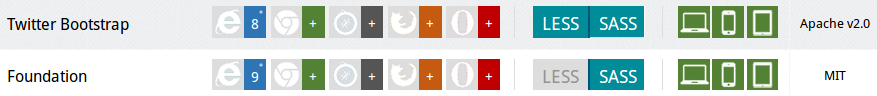
\includegraphics[scale=0.7]{images/Bootstrap&Foundation.png}
	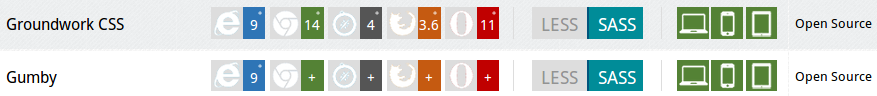
\includegraphics[scale=0.7]{images/Groundwork&Gumby.png} 
	
\includegraphics[scale=0.7]{images/Kube.png}  
	\caption[Framework Comparison]{Framework Comparison\footnote{\url{http://usablica.github.io/front-end-frameworks/compare.html}}}
	\label{img:Bootstrap&Foundation.png}
	\label{img:Groundwork&Gumby.png}   
	\label{img:Kube.png}                          
	\end{figure}

 Among all of the described above Web frameworks the most reasonable to chooose Twitter Bootstrap. It has all possible nowadays visualization modules, have been used for more than 1500+ sites, well-known among developers, reach API and examples, supported by all browsers, has a build-in fluid grid systems, that is simplify a lot building an cross-browser application.

\section{JavaScript MV* Frameworks}
	As was mentioned in the section 4.3.3, very important to realize loosely coupled system. Needs to be separated visualization of graphical modules on a web page from a code that is responsible for retrieving of a content. Thus was used AngularJS\footnote{AngularJS,\url{http://angularjs.org/}}. It is an open-source JavaScript framework, maintained by Google, that assists with running single-page applications. Its goal is to augment web-based applications with model–view–controller (MVC) capability, in an effort to make both development and testing easier.The library reads in HTML that contains additional custom tag attributes; it then obeys the directives in those custom attributes, and binds input or output parts of the page to a model represented by standard JavaScript variables. The values of those JavaScript variables can be manually set, or retrieved from static or dynamic JSON resources\cite{ wiki:angular}. AngularJS is a toolset for building the framework most suited to application development. It is fully extensible and works well with other libraries such as jQuery, on top of which was build XMPP. Every feature can be modified or replaced to suit unique development workflow and feature needs.

	AngularJS is built around the belief that declarative programming should be used for building user interfaces and wiring software components, while imperative programming is excellent for expressing business logic\footnote{What Is Angular?,\url{http://docs.angularjs.org/guide/introduction}}. The framework adapts and extends traditional HTML to better serve dynamic content through two-way data-binding(Figure 5.2) that allows for the automatic synchronization of models and views. As a result, AngularJS deemphasizes DOM manipulation and improves testability.

	\emph{Design goals}:
	\newline
	Decouple DOM manipulation from application logic. This improves the testability of the code. Decouple the client side of an application from the server side. This allows development work to progress in parallel, and allows for reuse of both sides.	Angular follows the MVC pattern of software engineering and encourages loose coupling between presentation, data, and logic components. Using dependency injection, Angular brings traditional server-side services, such as view-dependent controllers, to client-side web applications. Consequently, much of the burden on the backend is reduced, leading to much lighter web applications.

   \emph{Two-way data binding}
   \begin{figure}[!ht]
		\centering
		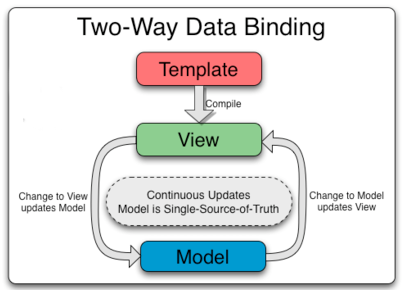
\includegraphics[scale=0.8]{images/2wayBinding.png}   
		\caption[Two-way data binding]{Two-way data binding\footnote{Angular JS Two-Way Data Binding,\url{http://docs.angularjs.org/guide/databinding}}}
		\label{img:interfaces}                           
		\end{figure}
	AngularJS two-way data binding is its most notable feature and reduces the amount of code written by relieving the server backend from templating responsibilities. Instead, templates are rendered in plain HTML according to data contained in a scope defined in the model. The \$scope service in Angular detects changes to the model section and modifies HTML expressions in the view via a controller. Likewise, any alterations to the view are reflected in the model. This circumvents the need to actively manipulate the DOM and encourages bootstrapping and rapid prototyping of web applications.

	The way Angular templates works is different, as illustrated on the Figure 5.3. They are different because first the template (which is the uncompiled HTML along with any additional markup or directives) is compiled on the browser, and second, the compilation step produces a live view. Any changes to the view are immediately reflected in the model, and any changes in the model are propagated to the view. This makes the model always the single-source-of-truth for the application state, greatly simplifying the programming model for the developer. View in such a way simply an instant projection of a model.
	    \begin{figure}[!ht]
		\centering
		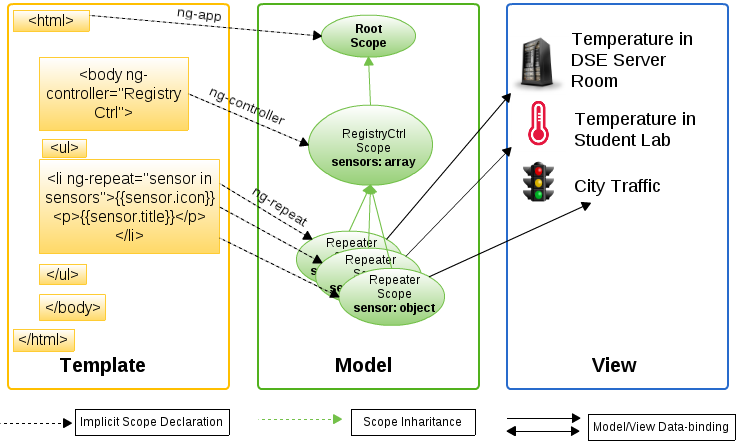
\includegraphics[scale=0.6]{images/3wayBinding.png}   
		\caption[Template Model View]{Template Model View}
		\label{img:interfaces}                           
		\end{figure}
        
    Because the view is just a projection of the model, the controller is completely separated from the view and unaware of it. As shown on the figure above, the resulting view can be applied to every data available ona  backend. Model handeler automaticaly generates a view for every new sensor. No need to change code or add new id and dependent handlers, variables, channels.
    The code realization of such a flow are shown on a listing~\ref{angular_template}
    \begin{lstlisting}[label=angular_template,caption=Template registry.html]
<div id="sensor_list">
    <div class="grid-sizer"></div>
    <div class="masonry-brick sensor-wrapper" id="{{sensor.id}}" ng-repeat="sensor in sensors | filter:{title: query}">
        <div class="sensor" ng-controller="SensorModalCtrl" ng-click="open()">
            <div class="icon">
                <img class="img-responsive" ng-src="{{sensor.icon}}">
                <h4>{{sensor.title}}</h4>
                <span class="label label-success" ng-show="user.check_subscribe(sensor.id)">Subscribed</span>
            </div>
            <div ng-show="sensor.picture">
                <img class="img-responsive" ng-src="{{sensor.picture}}">
            </div>
            <span class="description">{{sensor.description}}</span>
        </div>
    </div>
</div>
    \end{lstlisting}
    Model explicitly integrated to the HTML. As shown on the listing 5.1: ng-repeat,ng-src,ng-click and also variables {{sensor.*}}. Listin~\ref{angular_controller} shows controller implementation.

     \begin{lstlisting}[label=angular_controller,caption=Controller controller.js]
var sensdash_controllers = angular.module('sensdash.controllers', []);

sensdash_controllers.controller('RegistryCtrl', ['$scope', 'Sensor', 'User',
    function ($scope, Sensor, User) {
        $scope.sensors = Sensor.query();
        $scope.user = User;
}]);
    \end{lstlisting}
On the listing~\ref{angular_service} factory service, module of the AngularJS, parses REST API and creating sensors array based on factory pattern.
    \begin{lstlisting}[label=angular_service,caption=Controller controller.js]
var sensdash_services = angular.module('sensdash.services', ['ngResource']);

sensdash_services.factory('Sensor', ['$resource',
    function ($resource) {
        return $resource('api/sensors/:sensorId', {}, {
            query: {method: 'GET', params: {sensorId: 'all'}, isArray: true}
        });
    }]);
    \end{lstlisting}
\section{Twitter Bootstrap usage}


\section{Interface Implementation}
	 According to system architecture system has to implement two intefaces:
	 \begin{itemize}
	 \item Registry-Directory Manager
	 \item Data Hub-DataStream Handler and AuthHandler
	 \end{itemize}
	 XMPP connections live for arbitrarily long periods of time, but HTTP requests are quite short lived.
	A connection manager maintains an XMPP connection for a third party and provides access to the connection via the HTTP long polling technique.
	    \begin{figure}[!ht]
		\centering
		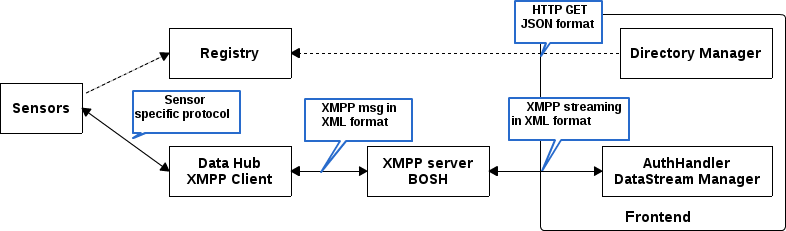
\includegraphics[scale=0.6]{images/XMPPflow.png}   
		\caption[XMPP BOSH/Stream]{XMPP interface flow}
		\label{img:interfaces}                           
		\end{figure}

	The browser and the connection manager communicate over HTTP using a simple protocol called BOSH. Essentially, BOSH helps an HTTP client establish a new XMPP session, then transports stanzas back and forth over HTTP wrapped in a special <body> element. It also provides some security features to make sure that XMPP sessions can’t be easily hijacked. The connection manager communicates with an XMPP server as if it were a normal client. In this way, an HTTP application can control a real XMPP session. Because of the efficiency and low latency afforded by the long polling technique, the end result performs quite well, rivaling native connections.

	XMPP connections are managed through the Strophe.Connection object. BOSH connection managers are exposed to HTTP clients as URLs, and the Strophe.Connection object you create needs to know about one of these URLs. Many XMPP servers come with support for BOSH built in, and they typically expose the service at http://example.com:5280/http-bind or http://example.com:5280/xmpp-httpbind . Some BOSH connection managers can handle communications for arbitrary XMPP servers, but generally the built-in connection managers can talk only to the server they run on. For developing the applications in this book, you are free to use the BOSH connection manager at http://bosh.metajack.im:5280/xmpp-httpbind . This BOSH connection manager is able to speak to any public XMPP server. This server is provided specifically for readers of this book to use during development to avoid everyone having to set up their own BOSH service.

	You can create a new Strophe.Connection object just as you would any other JavaScript object, by
using the new keyword~\ref{js_object}.	Once you have a connection object, you can call connect() and disconnect() to start and end	communication with the server::
\begin{lstlisting}[label=js_object,caption=Stanzas Format]
	var conn = new Strophe.Connection("http://bosh.likepro.co:5280/xmpp-httpbind");
	// starting a connection to example.com
	conn.connect("user@example.com", "mypassword", my_callback);
	// disconnecting
	conn.disconnect();
\end{lstlisting}
	The first two parameters to connect() are the JID and password to use to authenticate the session,
	and the last parameter is the callback function discussed earlier. The callback function will be called
	with a single parameter that is set to one of the statuses described in the previous section. A simple
	callback function that disconnects once the connection reaches the CONNECTED phase is shown here:
\begin{lstlisting}[label=js_object,caption=Stanzas Format]
	function my_callback(status) {
	if (status === Strophe.Status.CONNECTED) {
	 conn.disconnect();
	 }
    }
\end{lstlisting}
Every time the connection changes its status, this callback function is executed. The callback function simply ignores any status but the CONNECTED status, and disconnects once the connection
has reached that status.


\subsection{XEP-0060: Publish-Subscribe}
This specification defines an XMPP protocol extension for generic publish-subscribe functionality. The protocol enables XMPP entities to create nodes (topics) at a pubsub service and publish information at those nodes; an event notification (with or without payload) is then broadcasted to all entities that have subscribed to the node. Pubsub therefore adheres to the classic Observer design pattern and can serve as the foundation for a wide variety of applications, including news feeds, content syndication, rich presence, geolocation, workflow systems, network management systems, and any other application that requires event notifications\footnote{XEP-0049: Publish-Subscribe, \url{http://xmpp.org/extensions/xep-0060.html}}.

\subsubsection{Overview}
The XMPP publish-subscribe extension provides a framework for a wide variety of applications, including news feeds, content syndication, extended presence, geolocation, avatar management, shared bookmarks, auction and trading systems, workflow systems, network management systems, NNTP gateways, profile management, and any other application that requires event notifications.

This technology uses the classic "publish-subscribe" or "observer" design pattern: a person or application publishes information, and an event notification (with or without payload) is broadcasted to all authorized subscribers. In general, the relationship between the publisher and subscriber is mediated by a service that receives publication requests, broadcasts event notifications to subscribers, and enables privileged entities to manage lists of people or applications that are authorized to publish or subscribe. The focal point for publication and subscription is a "node" to which publishers send data and from which subscribers receive event notifications. Nodes can also maintain a history of events and provide other services that supplement the pure pubsub model. Figure 5.1
\begin{figure}[!ht]
    \centering
    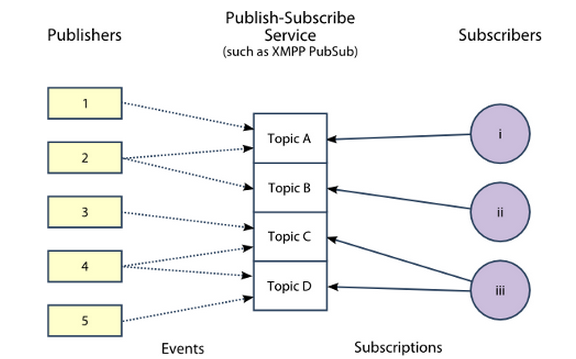
\includegraphics[scale=0.8]{images/XEP0049.png}   
    \caption[General Event Subscription]{General Event Subscription}
    \label{img:pub_sub}                           
    \end{figure}

The XMPP pubsub extension is similarly generic and is usable for a wide variety of purposes. It assumes nothing about the subscribers; they may be human, or they may be machines. Pubsub nodes, unlike multi-user chat rooms, are arranged in a tree-based hierarchy. One of the benefits of the tree shape is that entities can subscribe to non-leaf nodes of the tree, and events published below that node can also be received. Events can be published as notifications or as full payloads, and the subscriber can choose which is most appropriate. 
Retrieval of the publishing history is built in and fairly fine grained. The subscriber has more fine grained control over the delivery destination. The basic feature set of pubsub is quite easy to implement, and the core mechanics are quite simple to understand.
   
	\subsubsection{XMPP Pub-Sub flow}
	Although this specification is large because it defines many side use cases and possible error flows, the basic idea is simple:

	An entity publishes information to a node at a publish-subscribe service. The pubsub service pushes an event notification to all entities that are authorized to learn about the published information. Perhaps the most popular application of pubsub-like functionality is content syndication, which has become familiar from the RSS and Atom (RFC 4287\footnote{The Atom Syndication Format, \url{http://tools.ietf.org/html/rfc4287}}) feeds associated with weblogs, news sites, and other frequently-updated information available on the Internet. 
    \begin{figure}[!ht]
    \centering
    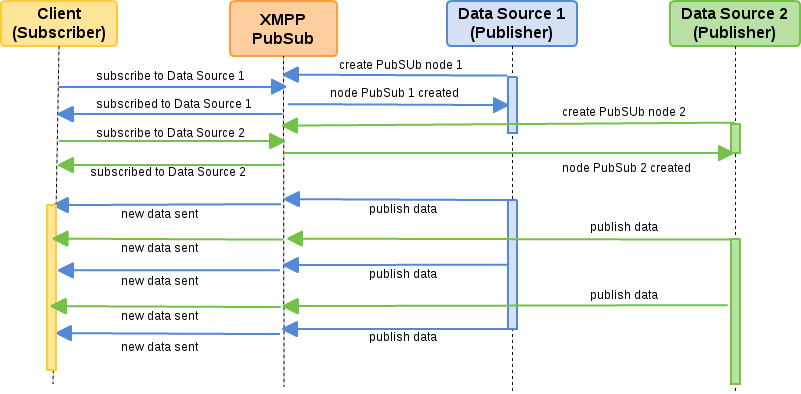
\includegraphics[scale=0.6]{images/PubSub.png}   
    \caption[Service PubSub]{Service PubSub}
    \label{img:pub_sub}                           
    \end{figure}

	Some example of code screenshot

	\subsubsection{XMPP Stanzas}
	Work is accomplished in XMPP by the sending and receiving of XMPP stanzas over an XMPP stream. Three basic stanzas make up the core XMPP toolset. These stanzas are <presence> , <message> , and <iq> . Each type of stanza has its place and purpose, and by composing the right kinds of quantities of these stanzas, sophisticated behaviors can be achieved. Remember that an XMPP stream is a set of two XML documents, one for each direction of communication. These documents have a root <stream:stream> element. The children of this <stream:stream> element consist of routable stanzas and stream related top-level children. Each stanza is an XML element, including its children. The end points of XMPP communication process input and generate output on a stanza-by-stanza basis.The following example shows a simplified and short XMPP session on listinf~\ref{stanzas}
		\begin{lstlisting}[label=stanzas,caption=Stanzas Format]
		<stream:stream>
			<iq type="get">
				<query xmlns="jabber:iq:roster"/>
			</iq>
			<presence/>

			<message to="darcy@pemberley.lit"
					 from="elizabaeth@longbourn.lit/chatroom"
			         type="chat">
			    <body>Hello chat room</body>
			</message> 

			<presence type="unavailable"/>
		</stream:stream>
		\end{lstlisting}

	In this example, Elizabeth created an XMPP stream by sending the opening <stream:stream> tag. With the stream open, she sent her first stanza, an <iq> element. This <iq> element requested Elizabeth’s roster, the list of all her stored contacts. Next, she notified the server that she was online and available with a <presence> stanza. After noticing that Mr. Darcy was online, she sent him a short <message> stanza, thwarting his attempt at small talk. Finally, Elizabeth sent another <presence> stanza to inform the server she was unavailable and closed the <stream:stream> element, ending the session.
    
    \subsubsection{Server}
	The set of XMPP servers that can mutually communicate forms an XMPP network. The set of public XMPP servers forms the global, federated XMPP network. If a server does not speak the server-to-server protocol, it becomes an island, unable to communicate with external servers. An XMPP server will usually allow users to connect to it. It is, however, also possible to write applications or services that speak the server-to-server protocol directly in order to improve efficiency by eliminating routing overhead. Anyone can run an XMPP server, and full-featured servers are available for nearly every platform. Ejabberd, Openfire, and Tigase are three popular open source choices that will work on Windows, Mac OS X, or Linux systems. Several commercial XMPP servers are available as well, including M-Link and Jabber XCP.
	
	\subsubsection{Connection}
	Before any stanzas are sent, an XMPP stream is necessary. Before an XMPP stream can exist, a connection must be made to an XMPP server. XMPP includes some sophisticated support for establishing connections to the right servers. Typically clients and servers utilize the domain name system (DNS) to resolve a server’s domain name into an address they can connect to. Email services in particular use mail exchange (MX) records to provide a list of servers that handle mail for a given domain so that one well-known server address does not have to handle every service. Email, being an early Internet application, got special treatment in DNS. These days, service records (SRV) are used to provide a similar function for arbitrary services. The first thing an XMPP client or server does when connecting to another XMPP server is to query the appropriate SRV record at the server’s domain. The response may include multiple SRV records, which can be used to load balance connections across multiple servers. If an appropriate SRV record cannot be found, the application tries to connect to the given domain directly as a fallback. Most libraries also allow you to specify a server to connect explicitly.
	\subsubsection{Long Polling}
	Even with AJAX, data was still being requested, or polled, at timed intervals. Servers can be crippled if too many clients poll too fast.However, to get quick updates, the polling interval needs to be quite small; the lowest latency possible is the length of the polling interval. Another issue with polling is that most poll requests do not receive new data. In order to see changes within a reasonable time frame of when they occur, the polling interval must be quite short, but the actual data may not change very often.
	For example, if there is new data ready on the server, the server answers immediately. If there is not new data, the server keeps the connection open, holding any reply. Once new data arrives, it finally responds to the request. If no new data arrives after some period of time, the server can send back an empty reply, so as not to hold too many open connections at once. Once a request is returned, the client immediately sends a new one, and the whole process starts over. Because each polling request is potentially open for a long period of time, this technique is called long polling. It has many advantages over normal polling.


\subsection{XEP-0049: Private XML Storage}
	A Jabber client can store any arbitrary XML on the server side by sending an <iq/> stanza of type "set" to the server with a <query/> child scoped by the 'jabber:iq:private' namespace. The <query/> element MAY contain any arbitrary XML fragment as long as the root element of that fragment is scoped by its own namespace. The data can then be retrieved by sending an <iq/> stanza of type "get" with a <query/> child scoped by the 'jabber:iq:private' namespace, which in turn contains a child element scoped by the namespace used for storage of that fragment. Using this method, Jabber entities can store private data on the server and retrieve it whenever necessary. The data stored might be anything, as long as it is valid XML\footnote{XEP0049 specification,\url{http://xmpp.org/extensions/xep-0049.html}}. One typical usage for this namespace is the server-side storage of client-specific preferences; 
	
	\subsubsection{Methods}
	\begin{figure}[!ht]
		\centering
		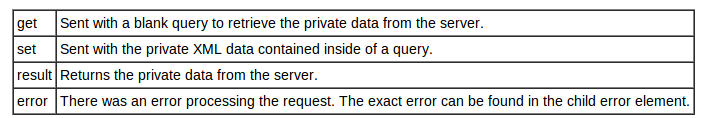
\includegraphics[scale=0.9]{images/xep0049Queries.png}   
		\caption[ Description of Acceptable Methods]{ Description of Acceptable Methods}
		\label{img:interfaces}                           
		\end{figure}
	\subsubsection{Elements}
	The root element of this namespace is query. At least one child element with a proper namespace must be included; otherwise the server must respond with a "Not Acceptable" error. A client must not query for more than one namespace in a single IQ get request. However, an IQ set or result may contain multiple elements qualified by the same namespace~\ref{client_save}.
    \begin{lstlisting}[label=client_save,caption=Client Stores Private Data]
	CLIENT:
	<iq type="set" id="1001">
	  <query xmlns="jabber:iq:private">
	    <exodus xmlns="exodus:prefs">
	      <defaultnick>Alice</defaultnick>
	    </exodus>
	  </query>
	</iq>

	SERVER:
	<iq type="result"
	    from="alice@likepro.co/"
	    to="alice@likepro.co/"
	    id="1001"/>
    \end{lstlisting}

     \begin{lstlisting}[label=client_load,caption=Client Retrieves Private Data]
		CLIENT:
		<iq type="get" id="1001">
		  <query xmlns="jabber:iq:private">
		    <exodus xmlns="exodus:prefs"/>
		  </query>
		</iq>

		SERVER:
		<iq type="result"
		    from="alice@likepro.co/"
		    to="alice@likepro.co/"
		    id="1001">
		  <query xmlns="jabber:iq:private">
		    <exodus xmlns="exodus:prefs">
		      <defaultnick>Alice</defaultnick>
		    </exodus>
		  </query>
		</iq>
    \end{lstlisting}

    The message format described above can be made by using two main functions: save(for saving data on the XMPP server) and load(to retrieve saved data from the XMPP server), as shown on the listing~\ref{save_load_ns}
	\begin{lstlisting}[label=save_load_ns,caption=Snippet of Save/Load preferences to a private namespace]
	      	save: function (property) {
	            xmpp.connection.private.set(property, property + ":ns", user[property], function (data) {
	                    console.log(property + " saved: ", data);
	                },
	                console.log);
	        },
	        load: function (property) {
	            xmpp.connection.private.get(property, property + ":ns", function (data) {
	                    user[property] = data != undefined ? data : [];
	                    if (property == 'subscriptions') {
	                        for (var i = 0; i < user.subscriptions.length; i++) {
	                            xmpp.subscribe(user.subscriptions[i]);
	                        }
	                    }
	                    $rootScope.$apply();
	                },
	        }
	\end{lstlisting}


\section{Browser Support}
	In past years a Flash-based media player in more than sufficient for streaming on the Web and this technology is still necessary to support legacy browsers. But thankfully modern standards have advanced and the inclusion of HTML5 video opens doors for dozens of new opportunities.

	In this guide I’d like to offer an introduction to HTML5 video for the Web. It will take some practice to understand the native in-browser player and all its functionality. When you’re working with a flash video player it’s all too common to associate all video formats in .flv. While this does work, most flv files cannot retain quality anywhere near the more advanced file formats/codecs. There are 3 important video types which are supported by HTML5: MP4, WebM, and Ogg/Ogv. The MPEG-4 file type is generally encoded in H.264 which allows for playback in third party Flash players. This means you don’t need to keep a .flv video copy to support a fallback method! WebM and Ogg are two much newer file types related to HTML5 video. Ogg uses Theora encoding which is based on the open-source standard audio file format. These can be saved with a .ogg or .ogv extension.
	So which of these file types do you need for your website? Well ideally all 3 would be great as they provide the full support spectrum. Yet this isn’t realistic, and in fact, you can cover all the bases with only two of them. Here is a breakdown of what works for each browser:

\subsection{3-tier Architecture in Software Projection}
\section{Use Case}
To demonstrate convincing scenario of usage SensDash as a user was choosen developer of a backend system. The implication that developer has sensors, which are connected to a single server with a DB.

 \subsection{Evaluation}
 By using temperature sensor from ACDSee project in TU Dresden which use XEP0045(Multi-user chat)instead of XEP0060.

\subsection{Summary}
This chapter presented details of implementation of the generic frontend prototype. Firstly, chosen tools and development environment were presented: jQuery, HTML5, CSS was used as a programming language, AngularJS together with Bootstrap was chosen for the web framework and Strophe.js was picked to implement the XMPP mechanism. Afterwards the interface flow by using XEP0060 and XEP0049 specification was implemented and described.

In this chapter the evaluation of the generic frontend prototype was performed. This was done by using convinsing scenario. 